La parte cruciale del progetto \emph{PathS} si basa sulla gestione delle informazioni aggiuntive relative ai percorsi pedonali e la possibilità di sfruttarle per fornire un servizio alternativo agli utenti finali. La persistenza, la gestione e l'elaborazione di questi dati avviene nella componente \emph{server}. 
In questo capitolo saranno presentati i requisiti individuati per assolvere allo scopo del progetto e il modo in cui questi requisiti hanno guidato la definizione dell'architettura del software da sviluppare.

\section{Requisiti}
Come per l'altra componente, anche nel caso del server si è preso spunto dalla precedente versione del progetto \emph{Path2.0} e si è cercato di identificarne i limiti per poter essere adattato al nuovo contesto e agli scopi più ampi che sono stati definiti. Le situazioni e le necessità a cui si intende applicare il progetto sono del tipo:
\begin{itemize}
\item qual è il percorso meno rumoroso in quest’ora del giorno?
\item che percorso devo seguire per ottenere il maggior numero di tratti all’ombra?
\item quali sono i percorsi preferiti dagli utenti che hanno visitato questa zona?
\end{itemize}
Le risposte fornite dovranno sempre tenere conto della soddisfabilità della domanda,quindi fornire sempre un percorso valido, ma valutare anche le preferenze espresse dall’utente.

Dal punto di vista tecnologico la soluzione precedente è stata valutata non idonea come base di partenza, in particolare presentava le seguenti caratteristiche che ne rendevano difficile una possibile evoluzione:
\begin{itemize}
\item il sistema era stato basato sul concetto dei percorsi accessibili e la ricerca del \emph{routing} esclusivamente come riutilizzo dei tratti noti con questa caratteristica;
\item vi è un forte accoppiamento e dipendenza dalle API Google Maps, i cui termini di utilizzo sono cambiati nel tempo e il modo in cui sono integrate è una forzatura inefficente ad esempio interrogazioni multiple per soddisfare una singola richiesta di routing;
\item il formato di comunicazione con il client era specifico e non adattabile al nuovo contesto senza una profonda rielaborazione;
\item il modello di persistenza delle informazioni non era adatto a gestire il nuovo \emph{set} di informazioni aggiuntive.
\end{itemize}

\begin{figure}[ht]
  \centering
  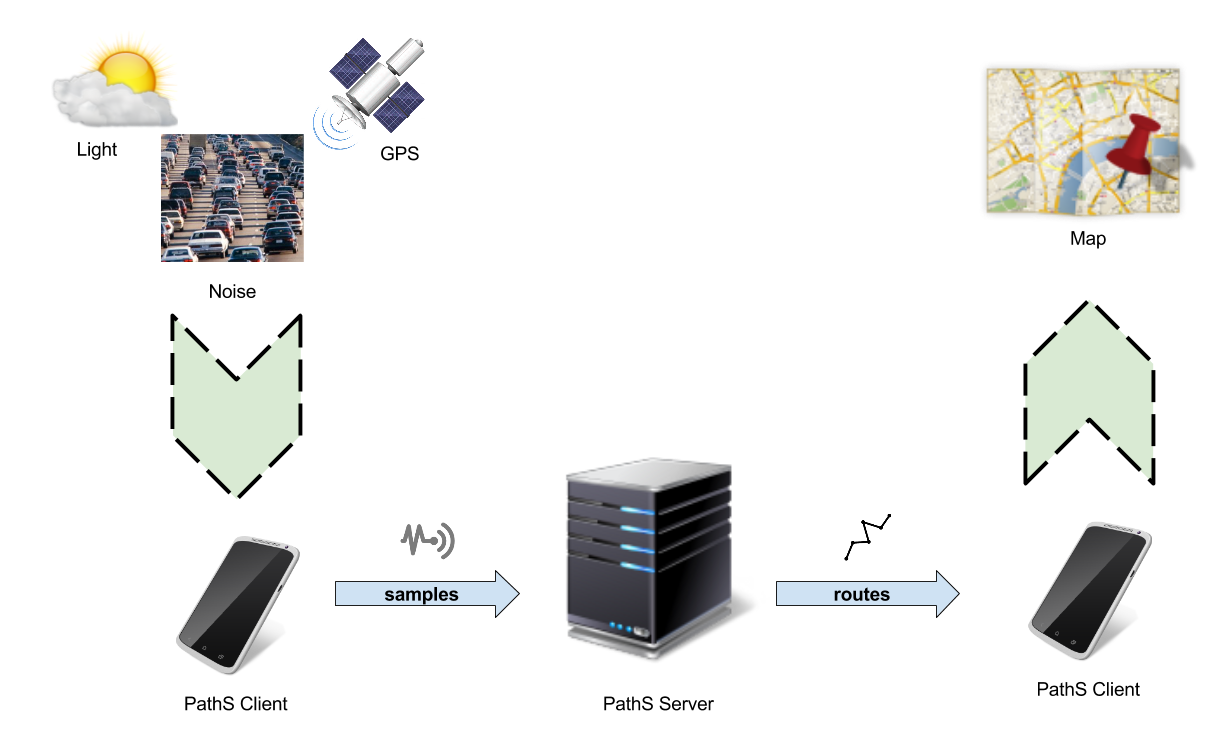
\includegraphics[width=\textwidth]{paths-general}
  \caption{\footnotesize{Schema generale del progetto PathS.}}
  \label{fig:paths-general}
\end{figure}

Considerati questi aspetti, ed in particolare le difficoltà nell'estendere il progetto esistente;  con il gruppo di lavoro si è cercato di ridefinire i requisiti del sistema ponendo l'attenzione su alcuni punti principali, ovvero:
\begin{itemize}
\item \textbf{raccolta campioni}: il sistema deve ricevere i campioni dalle applicazioni \emph{client} in un formato ben definito e dalle possibilità di estensione;
\item \textbf{persistenza}: il sistema deve memorizzare in modo efficiente e coerente le informazioni ricevute relative a campioni di diversa tipologia;
\item \textbf{associazione dei campioni ai percorsi}: il sistema deve eseguire l'operazione di associazione delle informazioni raccolte dai sistemi client (sensori) alle informazioni di geolocalizzazione e cartografia (tratti stradali);
\item \textbf{routing}: il sistema deve implementare un servizio di calcolo dei percorsi pedonali complesso che rielabori le informazioni precedentemente raccolte;
\item \textbf{interfacciamento con il client}: il sistema deve comunicare con le applicazioni \emph{mobile}  e i client \emph{desktop} fornendo le informazioni necessarie alla navigazione.
\end{itemize}

Uno schema ad alto livello del funzionamento previsto è presentato in figura \ref{fig:paths-general}.

Oltre ai requisiti fondamentali per il funzionamento del sistema, sono stati individuati altri criteri preferibili di carattere qualitativo da considerare nella progettazione e implementazione del software. Si possono riassumere in:
\begin{itemize}
\item \textbf{suddivisione delle responsabilità}: definire in modo specifico le funzioni svolte da ciascun componente del sistema, evitando elementi che svolgono funzioni troppo complesse o che accoppiano troppi elementi. Questo approccio consente una migliore testabilità delle sotto-componenti e la possibilità di rivedere e riprogettare alcuni dettagli senza dover manipolare l'intero prodotto software;
\item \textbf{astrazione}: identificare la funzione logica di ciascun componente concentrandosi sulla sua interfaccia prima di proseguire nell'implementazione. Questo consente di delineare con precisione il ruolo che dovrà svolgere, precondizioni,risultati attesi e i confini concettuali in cui opera. Rispettare questo criterio rende più facile lo sviluppo e il miglioramento dell'implementazione dei componenti senza doverne ridefinire la funzione logica e riducendo le ripercussioni sugli altri elementi dell'architettura;
\item \textbf{estensibilità}: rendere agevole sia in termini architetturali che implementativi la possibilità di migliorare ed estendere il sistema. L'obiettivo del progetto è stato volutamente limitato ad un primo risultato tangibile, considerando però che vi sia la possibilità di migliorare ed estendere le sue parti in modo facile e coerente con la base che si andrà a sviluppare.
\end{itemize}

\section{Componenti}
Basandosi sulle funzioni che deve svolgere il server, sono state identificate le componenti logiche principali da sviluppare. Per ciascun caso d'uso, si presenta in dettaglio il ruolo delle componenti e il modo in cui assolvono al raggiungimento del risultato.

\begin{figure}[ht]
  \centering
  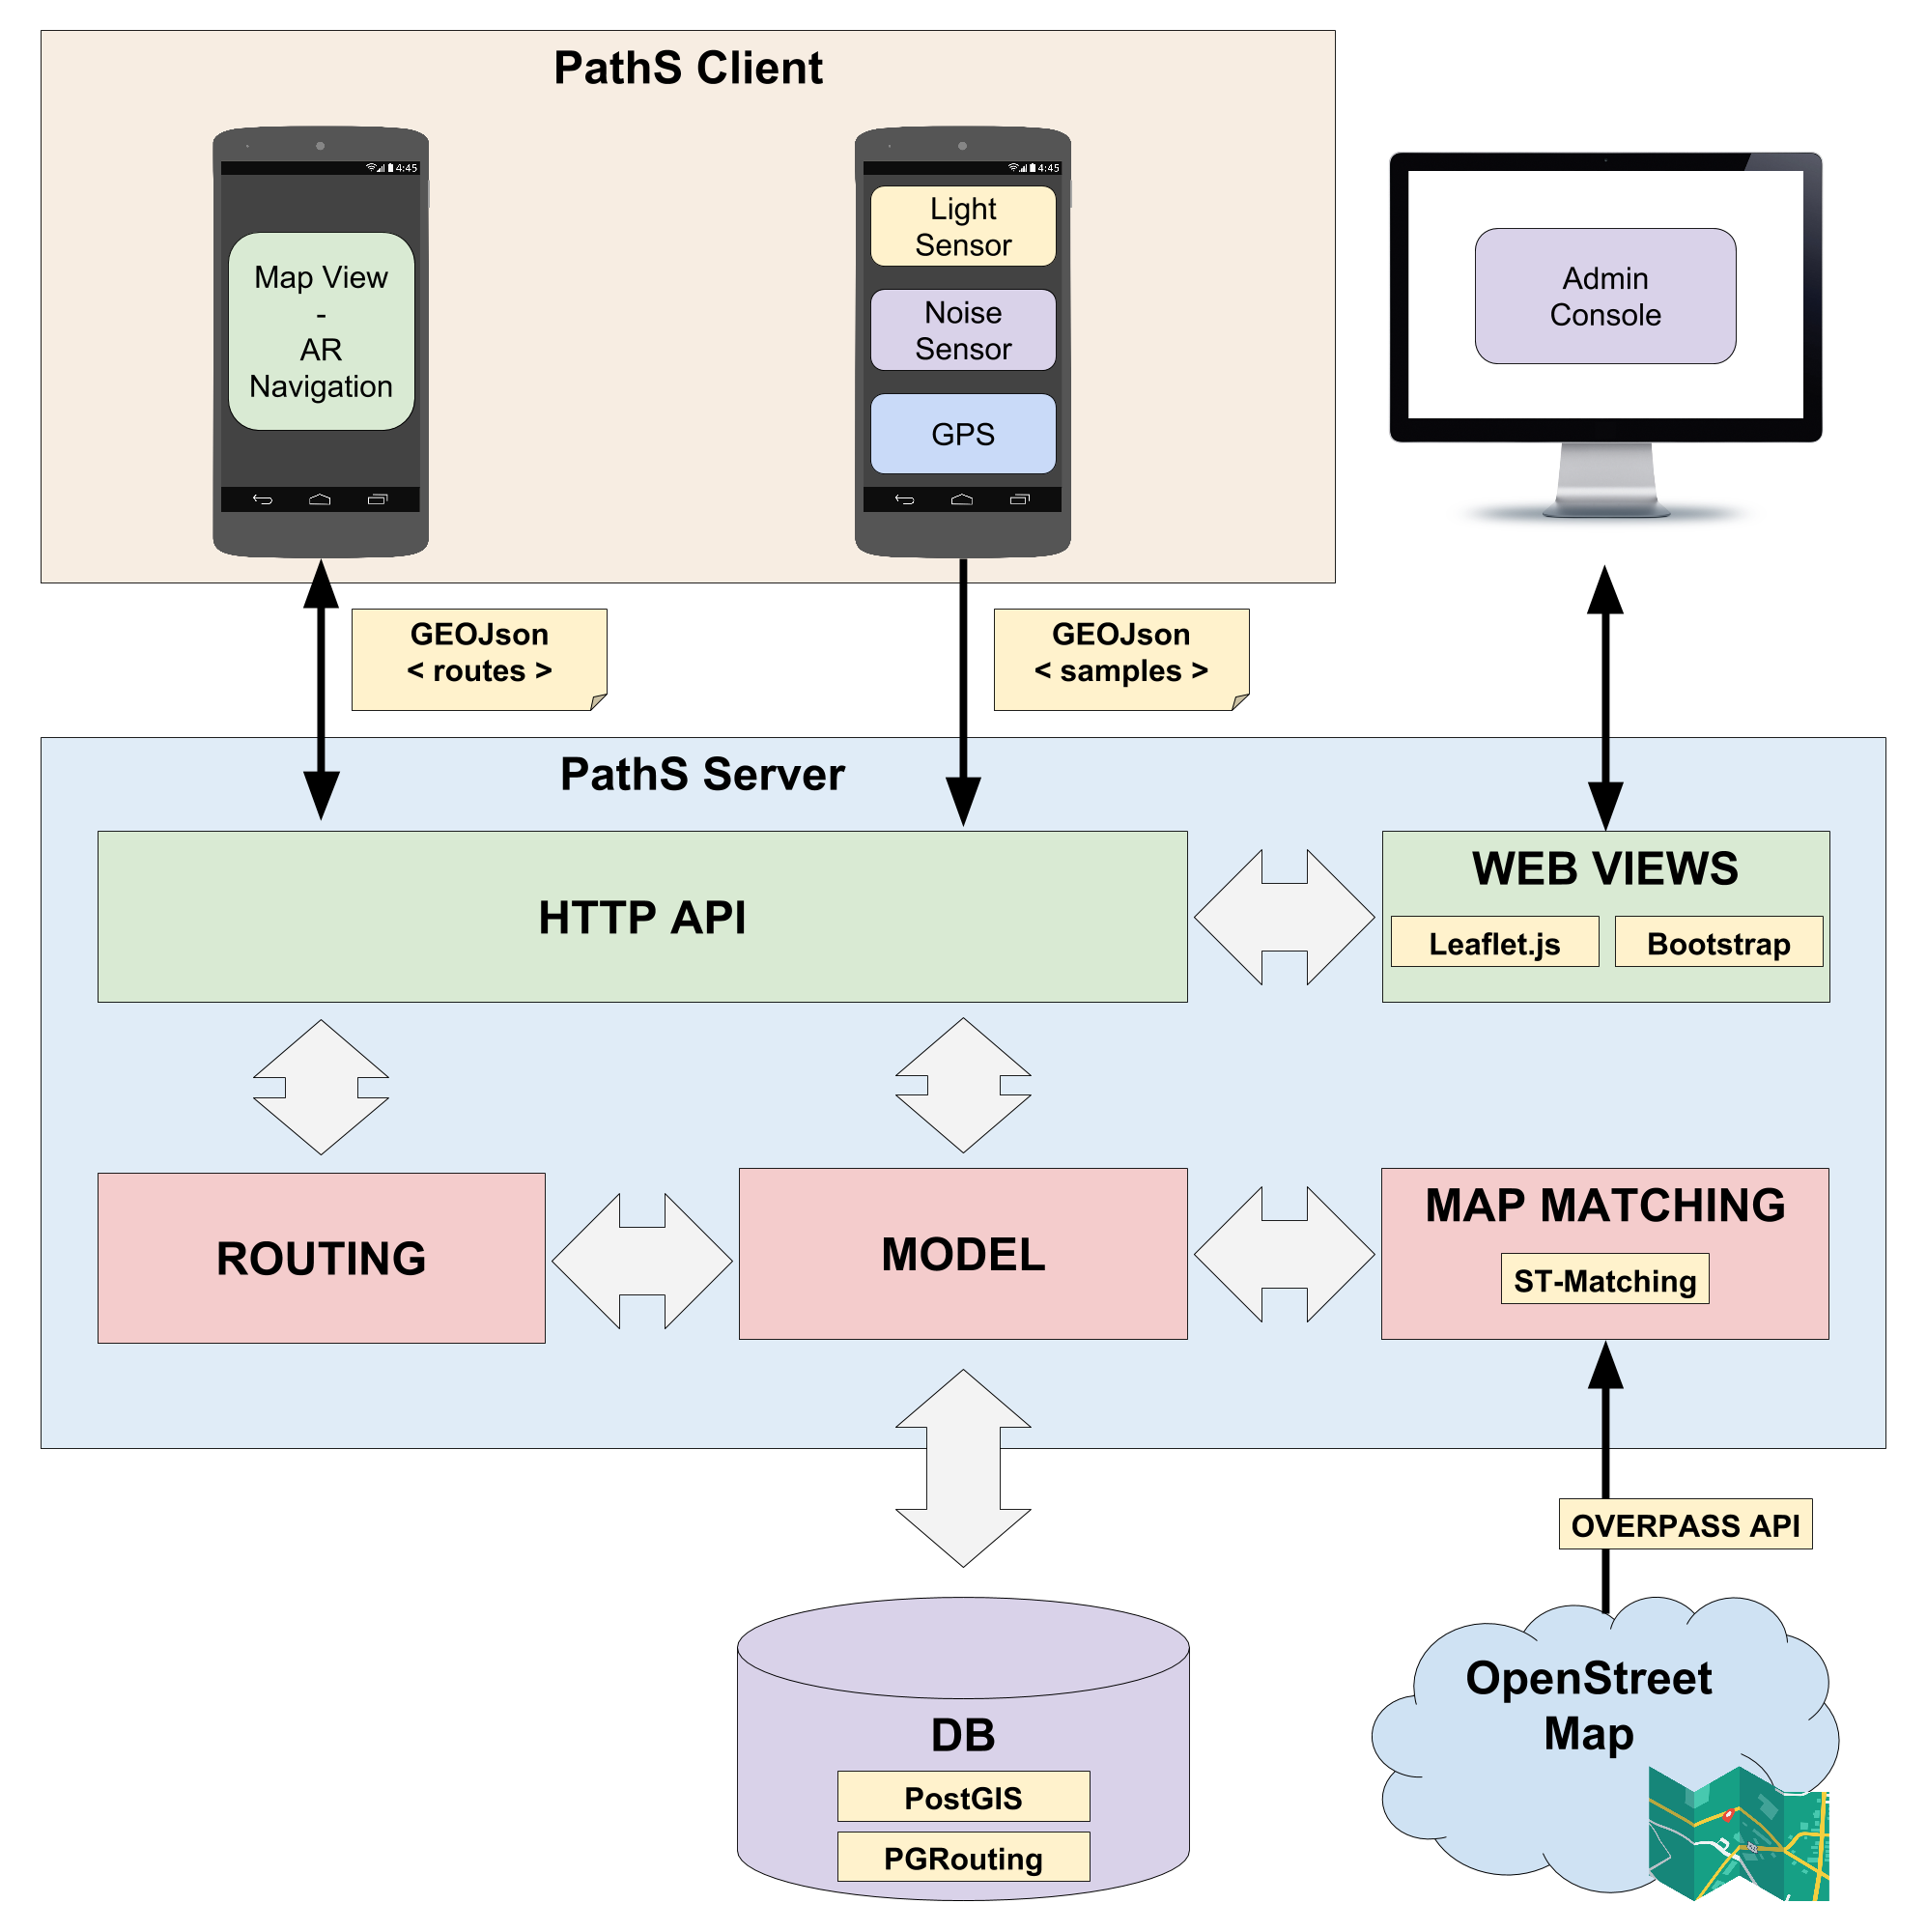
\includegraphics[width=\textwidth]{paths-componenti}
  \caption{\footnotesize{Macro componenti del del Server PathS.}}
  \label{fig:paths-componenti}
\end{figure}

\subsection{Ricezione dei campioni}
La prima componente che partecipa alla funzione di ricezione dei campioni deve dialogare con il client \emph{mobile}. Si è pensato di definire una \textbf{API} su protocollo \emph{HTTP} da utilizzare per tutte le chiamate di invio dati; in questo modo utilizzando un formato semplice che rispetta gli attuali \emph{standard de-facto}, risulta facilmente implementabile con qualsiasi tecnologia \emph{client} ed eventualmente da altre sorgenti dati future. Il componente \textbf{API} si occupa quindi di deserializzare i dati della richiesta e riorganizzarla per la persistenza. Il salvataggio avviene su apposito \textbf{Database} ma mediato da un componente intermedio di \textbf{Model}. Risultano quindi più agevoli le operazioni di interrogazione e persistenza, nonchè la leggibilità e semplicità dell'implementazione.

\subsection{Elaborazione dei campioni}
I campioni così come sono ricevuti dai client sono in formato grezzo e non consentono di sfruttare le inormazioni in esse contenute. Il passo principale per l'utilizzo dei dati è quello di associare ciascun dato ad un segmento della rete di trasporto. Tutto questo procedimento è sintetizzato con l'espressione \textbf{Map Matching} che è di fatto l'algoritmo che esegue tale associazione. Il \emph{matching} viene eseguito sia in modo autonomo dal server che tramite invocazioni dell'\textbf{API}. Il risultato delle esecuzioni dell'algoritmo viene comunque salvato a \textbf{database} tramite le apposite classi di \textbf{model}.

\subsection{Calcolo Percorsi}
Lo scopo pensato per l'utilizzo delle informazioni raccolte è quello di fornire servizi \emph{routing} alternativi, che tengano conto dei dati raccolti per suggerire percorsi che vanno oltre la semplice regola del percorso più breve. Per questo caso d'uso son quindi coinvolti i componenti:
\begin{itemize}
\item \textbf{API} per definire un formato con cui i client \emph{app} o \emph{browser} richiedono un percorso;
\item implementazione di un algoritmo di \textbf{routing} che esegue il calcolo effettivo;
\item l'algoritmo utilizzi le classi di \textbf{model} per accedere alle informazioni aggiuntive utilizzate nel calcolo.
\end{itemize}

\subsection{Accesso da Browser}
Per tutte le funzionalità principali del server si è pensato di dare un accesso di \emph{monitoraggio} tramite \emph{web browser}. In questo modo è possibile accedere facilmente alle informazioni gestite dal sistema, tramite visualizzazioni grafiche su mappa. La presentazione dei dati recuperati tramite le classi \textbf{model} è implementata con pagine \emph{html} e linguaggio \emph{Javascript} eseguito lato \emph{client}. Queste componenti possono essere raggruppate con la definizione di \textbf{view}.

\section{Tecnologie}
Per la realizzazione del progetto \emph{server} sono state selezionate alcune tecnologie e librerie utilizzate in modo trasversale per lo sviluppo dell'applicazione. I criteri adottati in questa scelta si riassumono in:
\begin{itemize}
\item preferenza per gli strumenti \emph{Open Source} facilitando accesso al software, la gestione delle licenze e lo sviluppo di eventuali modifiche;
\item preferenza per gli strumenti di larga adozione, per i quali sono disponibili \emph{on-line} documentazione ed esperienza diretta degli utenti,
\item preferenza per gli strumenti già adottati in altri progetti, in modo da ridurre i tempi di apprendimento e di configurazione.
\end{itemize}

Il risultato di questa selezione sono stati:
\begin{itemize}
\item \textbf{Framework Play!} \cite{playframework}: utilizzato per la struttura principale dell'applicazione Java. L'adozione di questo framework, già utilizzato in altre esperienze lavorative, ha permesso un rapido \emph{setup} dell'architettura \emph{Model-View-Controller} di base del server. Inoltre risultano semplificate alcune funzioni tra cui il \emph{mapping} delle richieste \emph{HTTP} previste dall'\emph{API}, la gestione della persistenza e l'\emph{Object Relational Mapping} tramite la specifica \emph{JPA} e l'implementazione \emph{Hibernate}. Il framework fornisce inoltre un facile motore di \emph{templating} per lo sviluppo delle pagine di presentazione.
\item \textbf{PostgresSQL} \cite{postgresql}: è il \emph{RDBMS} selezionato in quanto tra i prodotti open source più validi e diffusi allo stato attuale. Risulta inoltre particolarmente adatto con le funzioni \emph{GIS} aggiuntive fornite dalle librerie presentate in seguito e fondamentali per l'implementazione del progetto.
\item \textbf{LeafletJS} \cite{leafletjs}: libreria Javascript utilizzata per la presentazione delle mappe interattive. E' un prodotto open source altamente configurabile e di facile integrazione. E' risultato lo strumento ideale per presentare i dati in questa forma visuale senza legarsi ad altri servizi esterni. Supporta la visualizzazione da \emph{mobile} ed è particolarmente utile per la rappresentazione di \emph{layer} sovrapposti contenenti informazioni diverse.
\item \textbf{Bootstrap} \cite{bootstrap}: Uno dei framework \emph{HTML/CSS/JavaScript} più diffusi in assoluto, utilizzato per semplificare la realizzazione delle pagine web. Ha permesso la realizzazione di pagine web con \emph{design responsive} e graficamente gradevoli.
\end{itemize}
